\documentclass[12pt,a4paper]{article}
\usepackage[utf8]{inputenc}
\usepackage[siunitx,american]{circuitikz}
\usepackage{pgfplots}
\usepackage[margin=0.5in]{geometry}
\usepackage{textcomp}
\usepackage[spanish, es-tabla]{babel}
\usepackage{amsmath}
\usepackage{graphicx}
\usepackage[colorinlistoftodos]{todonotes}
\usepackage{amsmath}
\usepackage{tikz}
\usetikzlibrary{arrows}


\usepackage{parskip}
\usepackage{fancyhdr}
\usepackage{vmargin}
\setmarginsrb{3 cm}{2.5 cm}{3 cm}{2.5 cm}{1 cm}{1.5 cm}{1 cm}{1.5 cm}


\pgfplotsset{compat=1.15}

\begin{document}
\section{Ejercicio I}
\subsection{Analisis del circuito}
En este ejercicio se analizo el circuito \ref{fig:circuito_1}. 

\begin{figure}[ht]                                                       
    \centering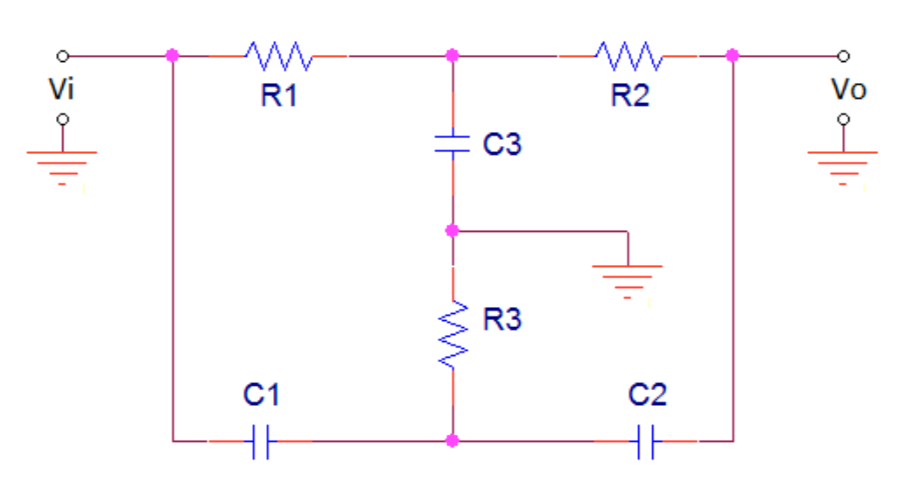
\includegraphics[width=0.8\textwidth]{circuito_1.png}
    \caption{Filtro Notch Pasivo}
    \label{fig:circuito_1}
    \end{figure}


En primer lugar, se calculo analíticamente al circuito mediante un método alternativo como es el de cuadripolos para
obtener la función transferencia $H(s)$ que se puede ver en la ecuación \ref{transferencia_1}. Vale aclarar que se tomo la ayuda propuesta por la catedra y se considero que $R_{1}$ = $R_{2}$
= $2R_{3}$, $2C_{1} = 2C_{2} = C_{3}$

\begin{equation} H(s) = \frac{(\frac{S}{1/C_{3} R_{3}})^2 + 1} {(\frac{S}{1/C_{3}R_{3}})^2 + 4\frac{S}{C_{3}R_{3}} + 1}  \label{transferencia_1}\end{equation}

Como se puede observar, la función transferencia describe un filtro Notch. Su frecuencia de corte es
$Wc$. Su expresión se muestra en la ecuación \ref{frecuencia_corte}

\begin{equation} W_{0} =  \frac{1}{C_{3} R_{3}}  \label{frecuencia_corte}\end{equation}

La frecuencia de corte pedida es $10.8k Hz$. Entonces nos queda la relación que se puede ver en la ecuación 
\ref{relacion_RC}.

\begin{equation} R_{3} = \frac{1}{C_{3} 2\pi 10.8k} \label{relacion_RC}\end{equation}

Para obtener la respuesta inpulsiva $h(t)$, se utilzo la antitrasformada de Laplace. Esta resulto ser: 

\begin{equation} h_{t} = asdasd  \end{equation}




Volviendo a la relación \ref{relacion_RC} es posible dar valores a la capacitor y asi obtener un valor para las resistencias. Teniendo en cuenta
los valores comerciales disponibles en el pañol, se tomo $C_{3} = 10nF$ por lo que se obtuvo $R_{3}=1.47k\Omega$. Como
no hay disponible una resistencia de ese valor, se utilizo $R_{3}=1.5k\Omega$. Tampoco se encontraron capacitores de $C = 5nF$ 
por lo que $C_{1} = 4.7nF$ y  $C{2} = 4.7nF$. Estos valores se cargaron en LTspice y se obtuvo el bode de la 
figura \ref{fig:bode_ltspice_teorico}.

\begin{figure}[ht]                                                       
    \centering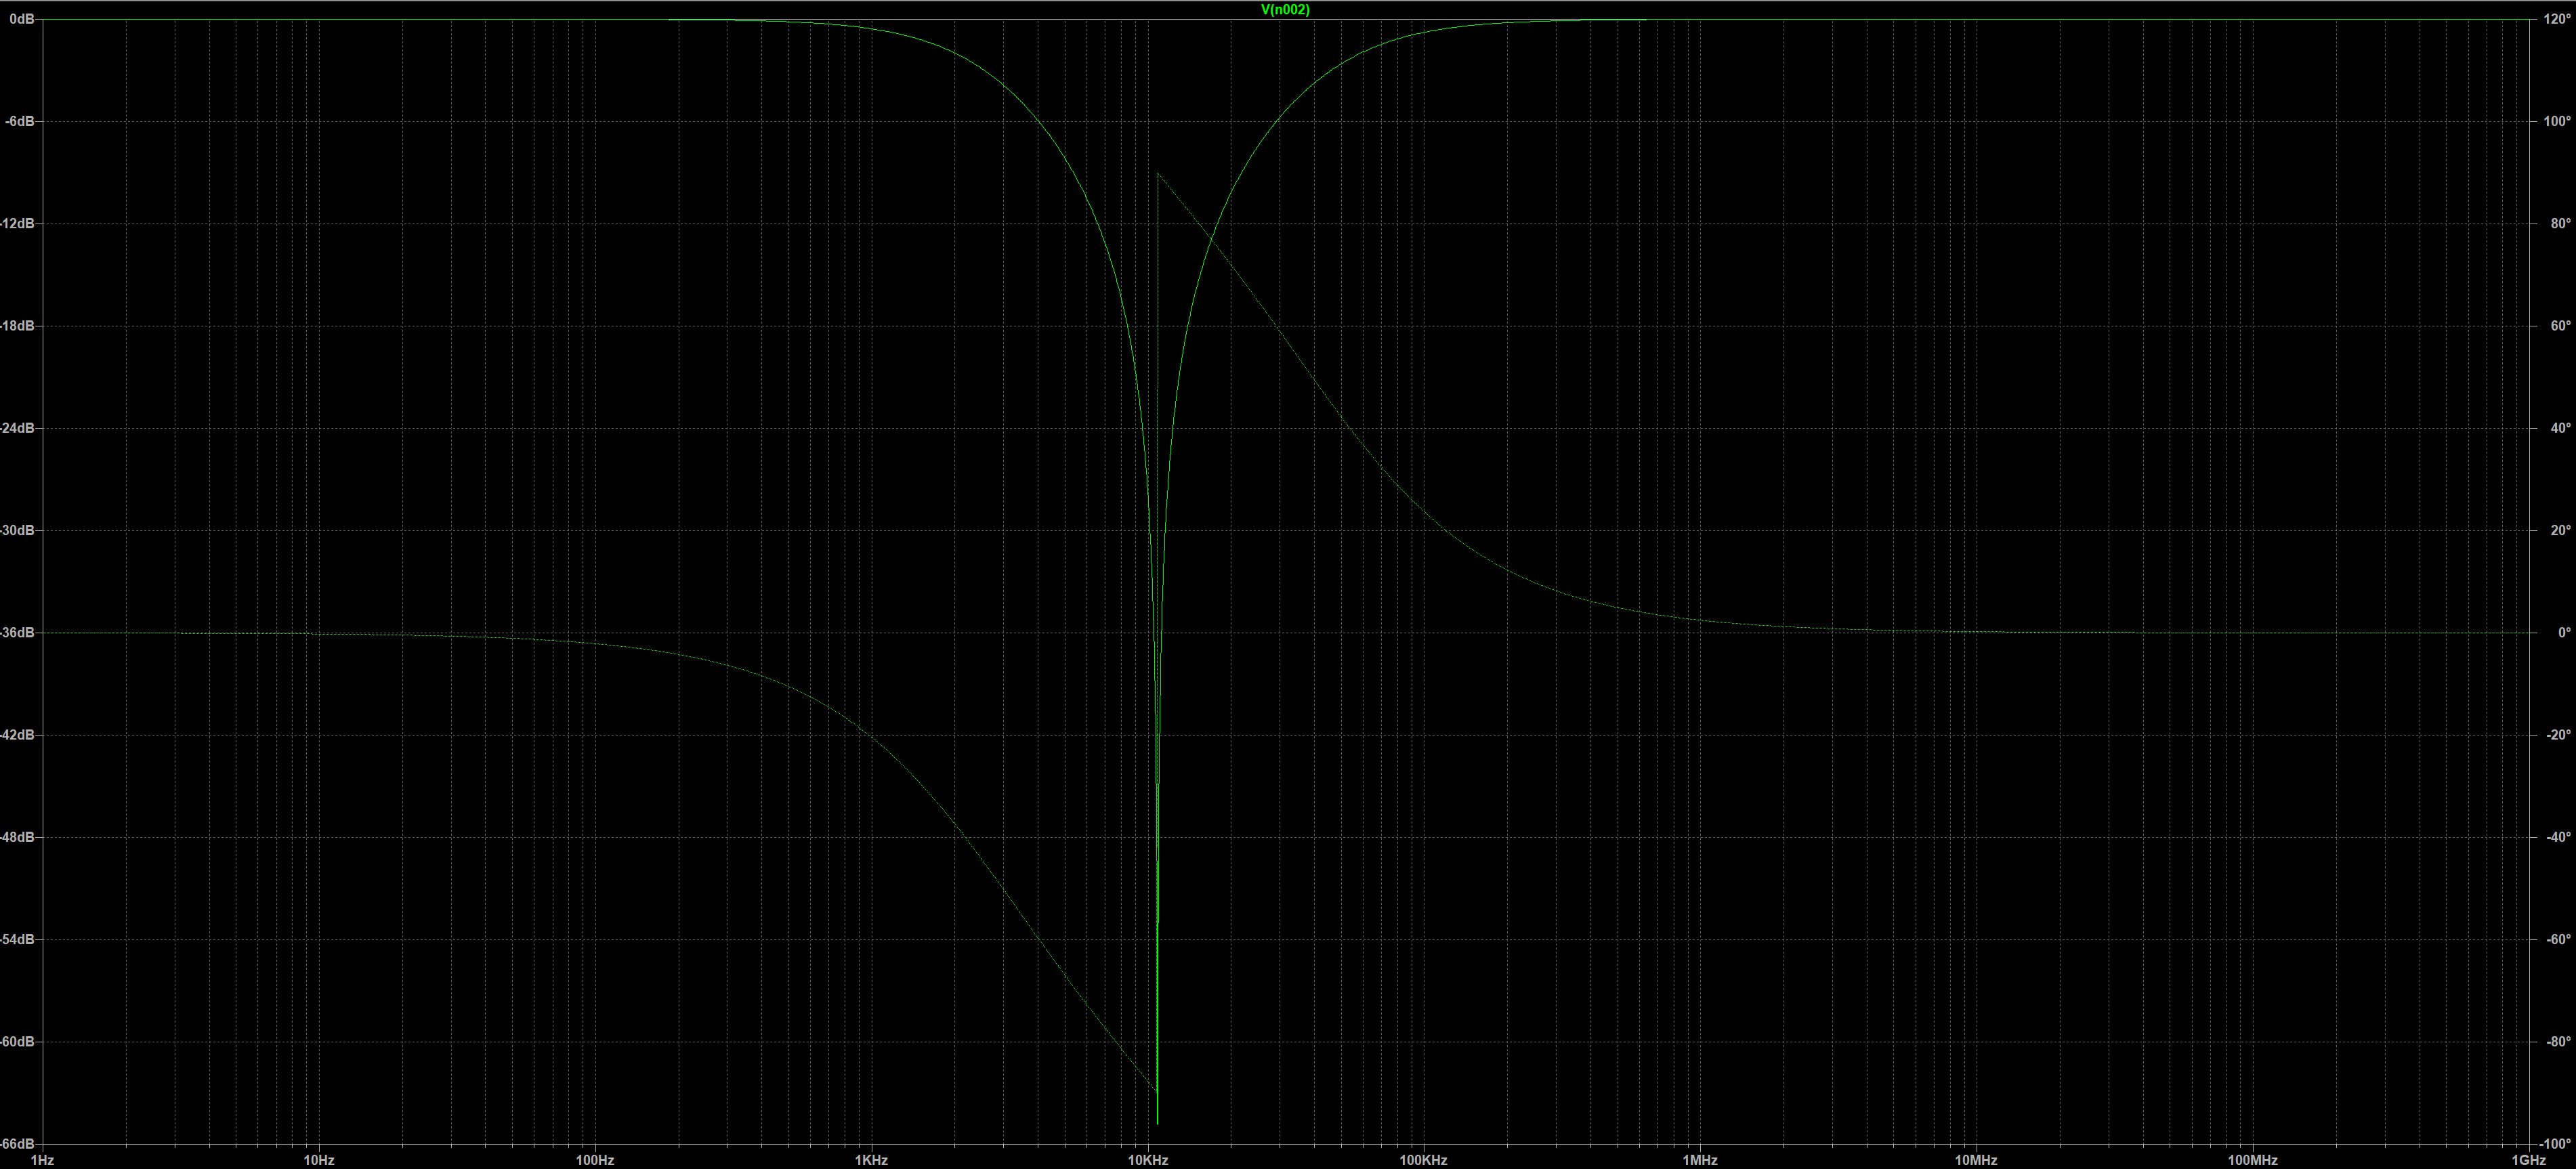
\includegraphics[width=0.8\textwidth]{bode_ltspice_teorico.png}
    \caption{Circuito con los componentes definidos}
    \label{fig:bode_ltspice_teorico}
    \end{figure}

Se puede observar que el comportamiento del bode describe un filtro notch y que la frecuencia de corte se ubica en $11.1kHz$. Si
bien la frecuencia de corte pedida es $10.8kHz$ nos vemos obligados a tomar $11.1kHz$ por motivos de disponibilidad de componentes
en el pañol. Luego las futuras mediciones se comparan respecto al bode obtenido en la figura \ref{fig:bode_ltspice_teorico}. \\

Para poder terminar de caracterizar el sistema hace falta el diagrama de polos y ceros. Los polos y ceros
se obtienen facilmente si reordenamos la funcion trasferencia como se ve continuación:

\begin{center}
    $H(S) = \frac{(S-S_{1})(S-S_{2})}{(S-P_{1})(S-P_{2})S}$  \\
\end{center}

Hay dos ceros:
\begin{center}
    $S_{1}=69743.35691j $
    $S_{2}=-69743.35691j $
    \end{center}

Hay dos polos:

\begin{center}
    $P_{1}=-18687.67616$
    $P_{2}=-260285.7515$
\end{center}

Como se puede ver los dos ceros se encuentran sobre el eje imaginario y los dos polos en el eje real del
semilado negativo


\begin{center}\begin{tikzpicture}
    \draw   (5,0) -- (-5, 0)
            (0,5) -- (0,-5);
    \draw   [red, thick](0,0) -> (0,4.5) node[anchor=north east] {S1};
    \draw   [red, thick](0,0) -> (0,-4.5) node[anchor=north east] {S2};
    \draw   [blue, thick](0,0) -> (-1,0) node[anchor=north east] {P1};
    \draw   [blue, thick](0,0) -> (-2,0) node[anchor=north east] {P2};
    \end{tikzpicture}
    \end{center}

\subsection{Respuesta en frecuencia}
Con los valores de los componentes calculados anteriormente, se diseño una placa en Altium. Su diseño se 
puede ver en la figura \ref{fig:placa_altium}

%\begin{figure}[ht]                                                       
%    \centering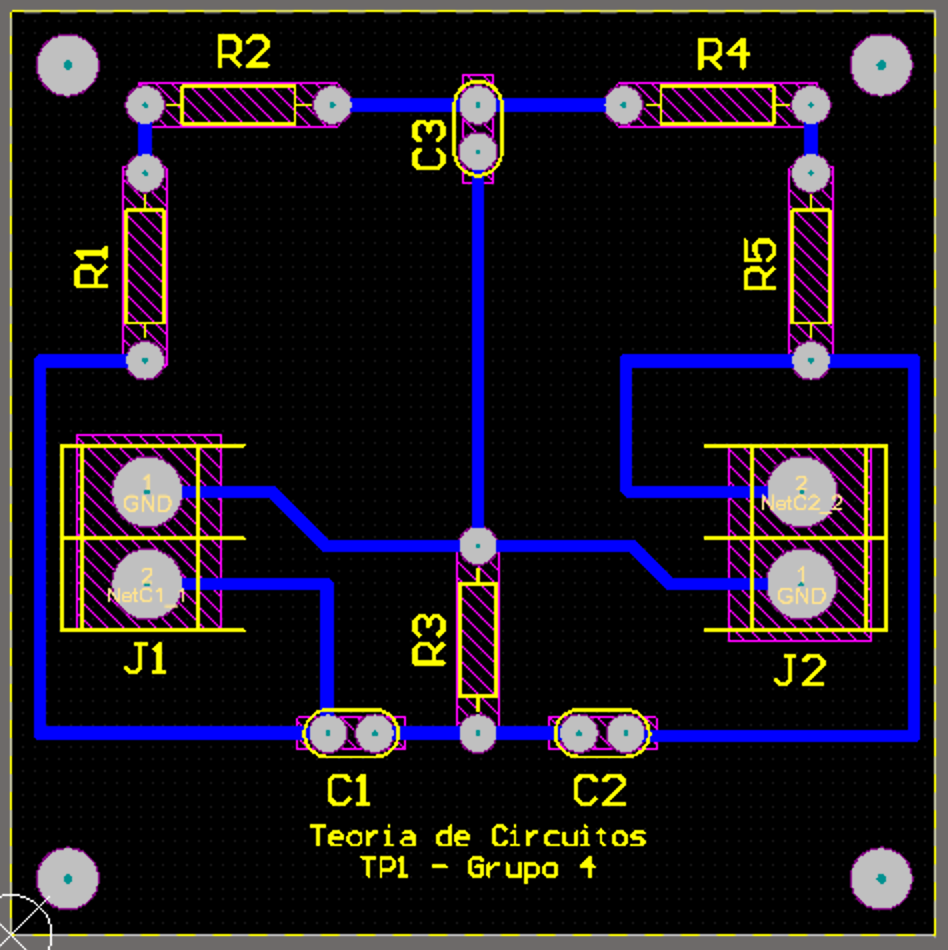
\includegraphics[width=0.8\textwidth]{placa_altium.png}
%    \caption{Filtro Notch Pasivo}
%    \label{fig:placa_altium}
%    \end{figure}

Notar que se tuvieron que utilizar dos resistencias en serie de $1.5k\Omega$ para obtener una
resistencia de $5k\Omega$. 

Para medir la respuesta en frecuencia se utilizo una senoide de $10V$ pico a pico en $V_{in}$ y se midió $V_{out}$
con la ayuda de un osciloscopio . Los resultados se pueden ver en la figura \ref{fig:rta_frec}







\subsection{Respuesta al escalón}
En esta parte se analizo la respuesta al escalon. En primer lugar se calculo la expresion analitica. Teniendo en cuenta que 
la entreda $X(t)$ es el escalon $U(t)$, que su transformada de Laplace es $\frac{1}{S}$ y que la funcion transferencia es la que 
vimos en la ecuacion \ref{transferencia_1}. La transformada de Laplace de la salida nos queda \ref{transferencia_2}


\begin{equation} Y(S) = \frac{S^2+W_{0}^2}{S^2+4W_{0}S+W_{0}^2} * \frac{1}{S}  \label{transferencia_2}\end{equation}

Si acomodamos un poco esta expresion podemos llegar a: \\

\begin{center}
    $Y(S) = \frac{(S-S_{0})(S+S_{0})}{(S-P_{1})(S-P_{2})S}$  \\
    
    $S_{0}=69743.35691j
    P_{1}=-18687.67616
    P_{2}=-260285.7515$
    \end{center}

Si antitrasformamos nos queda:\\

\begin{center}
    $y(t) = (A\exp{P_{1}t}+B\exp{P_{2}t}+C) * u(t)$

    $A = \frac{P_{1}^2 + W_{0}^2}{(P_{1}-P_{2})*P_{1}} = -1.1547$
    $B = \frac{P_{2}^2 + W_{0}^2}{(P_{2}-P_{1})*P_{2}} =  1.1547$
    $C = \frac{W_{0}^2}{(P_{2}P_{1}} = 1$

    \end{center}

%Si simulamos en LTspice la respuesta al ecalon tomando $C_{3} = 10nF$ y $R_{3}=1.47k\Omega$, nos queda los que observamos en 
%la figura \ref:fig{rta_escalon_teorica}

%\begin{figure}[ht]                                                       
%    \centering\includegraphics[width=0.8\textwidth]{rta_escalon_teorica.png}
%    \caption{Respuesta al Escalón}
%    \label{fig:rta_escalon_teorica}
%    \end{figure}

Las mediciones resultaron ser:

\end{document}